\documentclass[11pt,a4paper]{article}
%%%%%%%%%%%%%%%%%%%%%%%%% Credit %%%%%%%%%%%%%%%%%%%%%%%%

% template ini dibuat oleh martin.manullang@if.itera.ac.id untuk dipergunakan oleh seluruh sivitas akademik itera.

%%%%%%%%%%%%%%%%%%%%%%%%% PACKAGE starts HERE %%%%%%%%%%%%%%%%%%%%%%%%
\usepackage{graphicx}
\usepackage{caption}
\captionsetup[table]{name=Tabel}
\captionsetup[figure]{name=Gambar}
\usepackage{tabulary}
% \usepackage{amsmath}
\usepackage{fancyhdr}
% \usepackage{amssymb}
% \usepackage{amsthm}
\usepackage{placeins}
% \usepackage{amsfonts}
\usepackage{graphicx}
\usepackage[all]{xy}
\usepackage{tikz}
\usepackage{verbatim}
\usepackage[left=2cm,right=2cm,top=3cm,bottom=2.5cm]{geometry}
\usepackage{hyperref}
\hypersetup{
    colorlinks,
    linkcolor={red!50!black},
    citecolor={blue!50!black},
    urlcolor={blue!80!black}
}
\usepackage{libertine}
\usepackage{libertinust1math}
\usepackage[T1]{fontenc}
\usepackage{inconsolata}

\usepackage{caption}
\usepackage{subcaption}
\usepackage{multirow}
\usepackage{psfrag}
\usepackage[T1]{fontenc}
\usepackage[scaled]{beramono}
% Enable inserting code into the document
\usepackage{listings}
\usepackage{xcolor} 
% custom color & style for listing
\definecolor{codegreen}{rgb}{0,0.6,0}
\definecolor{codegray}{rgb}{0.5,0.5,0.5}
\definecolor{codepurple}{rgb}{0.58,0,0.82}
\definecolor{backcolour}{rgb}{0.95,0.95,0.92}
\lstdefinestyle{mystyle}{
	backgroundcolor=\color{backcolour},   
	commentstyle=\color{green},
	keywordstyle=\color{codegreen},
	numberstyle=\tiny\color{codegray},
	stringstyle=\color{codepurple},
	basicstyle=\ttfamily\footnotesize,
	breakatwhitespace=false,         
	breaklines=true,                 
	captionpos=b,                    
	keepspaces=true,                 
	numbers=left,                    
	numbersep=5pt,                  
	showspaces=false,                
	showstringspaces=false,
	showtabs=false,                  
	tabsize=2
}
\lstset{style=mystyle}
\renewcommand{\lstlistingname}{Kode}
%%%%%%%%%%%%%%%%%%%%%%%%% PACKAGE ends HERE %%%%%%%%%%%%%%%%%%%%%%%%


%%%%%%%%%%%%%%%%%%%%%%%%% Data Diri %%%%%%%%%%%%%%%%%%%%%%%%
\newcommand{\stuid}{120140154}
\newcommand{\student}{\textbf{Ryan Ernanda (\stuid{})}}
\newcommand{\course}{\textbf{Sistem Operasi-RB (IF2223)}}
\newcommand{\assignment}{\textbf{1}} % tugas ke...

%%%%%%%%%%%%%%%%%%% using theorem style %%%%%%%%%%%%%%%%%%%%
\newtheorem{thm}{Theorem}
\newtheorem{lem}[thm]{Lemma}
\newtheorem{defn}[thm]{Definition}
\newtheorem{exa}[thm]{Example}
\newtheorem{rem}[thm]{Remark}
\newtheorem{coro}[thm]{Corollary}
\newtheorem{quest}{Question}[section]
%%%%%%%%%%%%%%%%%%%%%%%%%%%%%%%%%%%%%%%%
\usepackage{lipsum}%% a garbage package you don't need except to create examples.
\usepackage{fancyhdr}
\usepackage[ddmmyyyy]{datetime}
\pagestyle{fancy}
\lhead{Ryan Ernanda (120140154)}
\rhead{ \thepage}
\cfoot{\textbf{HandsOn 1 : Working With Linux}} % ini untuk judul tugas
\renewcommand{\headrulewidth}{0.4pt}
\renewcommand{\footrulewidth}{0.4pt}

%%%%%%%%%%%%%%  Shortcut for usual set of numbers  %%%%%%%%%%%

\newcommand{\N}{\mathbb{N}}
\newcommand{\Z}{\mathbb{Z}}
\newcommand{\Q}{\mathbb{Q}}
\newcommand{\R}{\mathbb{R}}
\newcommand{\C}{\mathbb{C}}
\setlength\headheight{14pt}

%%%%%%%%%%%%%%%%%%%%%%%%%%%%%%%%%%%%%%%%%%%%%%%%%%%%%%%555

\begin{document}
\thispagestyle{empty}
\begin{center}
	
\includegraphics[scale = 0.15]{Gambar/ifitera-header.png}
	\vspace{0.1cm}
\end{center}
\noindent
% change font family for header section only
%{\fontfamily{LinuxLibertineT-OsF}\large\selectfont 
{\large
\rule{17cm}{0.2cm}\\[0.3cm]
Nama: \student \hfill Tugas Ke: \assignment\\[0.1cm]
Mata Kuliah: \course \hfill Tanggal: \today\\
\rule{17cm}{0.05cm}
\vspace{0.1cm}
}


%%%%%%%%%%%%%%%%%%%%%%%%%%%%%%%%%%%%%%%%%%%%% BODY DOCUMENT %%%%%%%%%%%%%%%%%%%%%%%%%%%%%%%%%%%%%%%%%%%%%
\section{Tujuan Hands On}
    Tujuan dari tugas Hands On 1 adalah untuk memperkenalkan linux versi Ubuntu 20.04.3 LTS (64-bit) serta memahami dari perintah perintah dasar linux seperti echo, man, grep, sed, ls, mkdir, rmdir, rm, chmod, nano, cat, cp, cd, mv, dan lain lain.

\section{Spesifikasi Sistem}
    Perangkat lunak yang saya gunakan sebagai virtual dari sistem operasi adalah \textit{Oracle VM VirtualBox} versi 6.1, dan spesifikasi dari sistem operasi linux Ubuntu yaitu 2 GB RAM, 13 GB \textit{storage}, 16 MB VRAM, 1 CPU \textit{Processors}. 
    \begin{figure}[h]
    \centering
    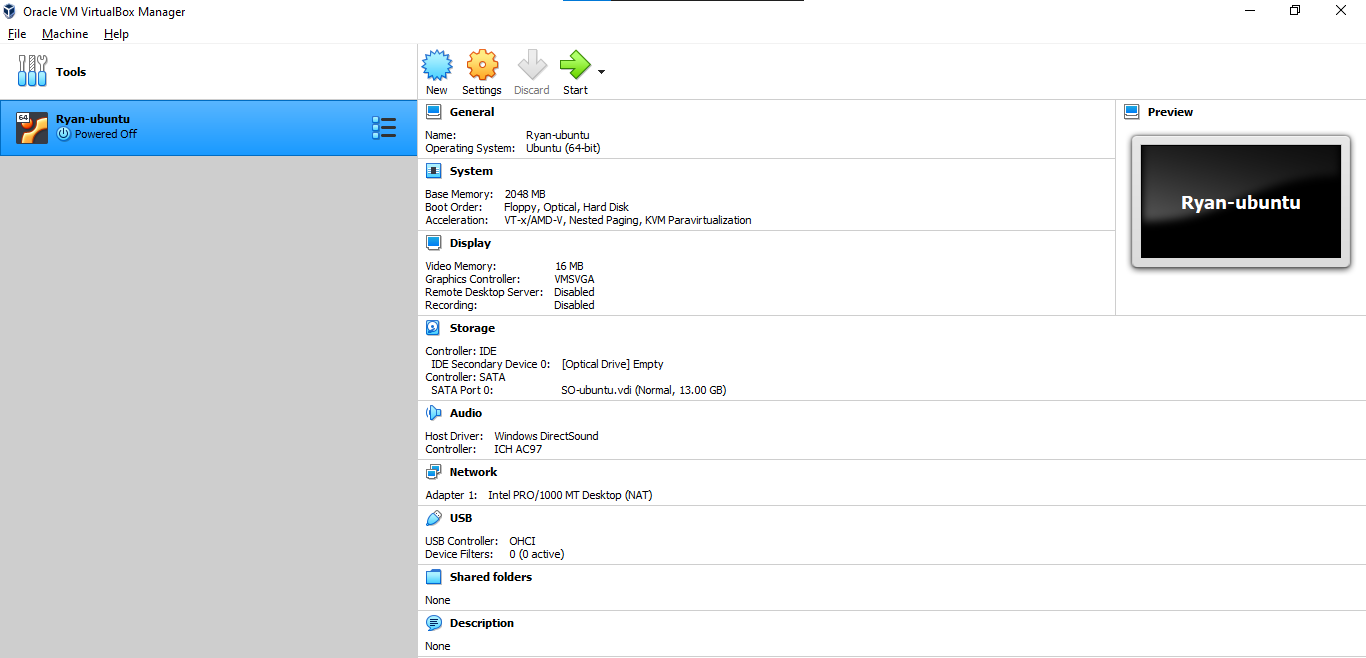
\includegraphics[width=0.8\textwidth]{Gambar/Spek.png}
    \caption{Spesifikasi Sistem Operasi}
    \label{fig:my_label}
    \end{figure}

\section{Laporan Percobaan Tut1}
\subsection{Tut 1.1 Echo}
    Percobaan tut 1.1 menampilkan kata dengan \textit{syntax: echo} yaitu \textit{"hello world"}, echo ini memiliki fungsi yaitu mencetak atau menampilkan string pada Terminal.
    \begin{figure}[h]
    \centering
    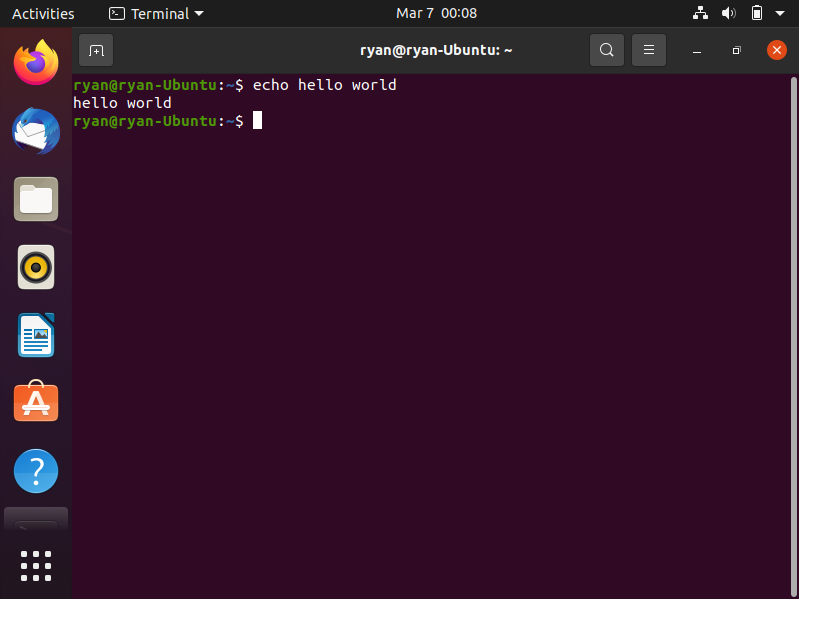
\includegraphics[width=0.5\textwidth]{Gambar/tut 1.1 echo.png}
    \caption{Echo Hello World}
    \label{fig:my_label}
    \end{figure}
    \newpage
    
\subsection{Tut 1.2 Man}
     Percobaan tut 1.2 menampilkan fungsi dari sebuah \textit{command} dengan \textit{syntax man}. man merupakan \textit{command} yang befungsi dalam menampilkan suatu fungsi dari \textit{command} lain. saya menggunakan man ls, ini berfungsi menampilkan kegunaan dari perintah ls serta penjelasan \textit{syntax} mendetail.
     \begin{figure}[h]
     \centering
    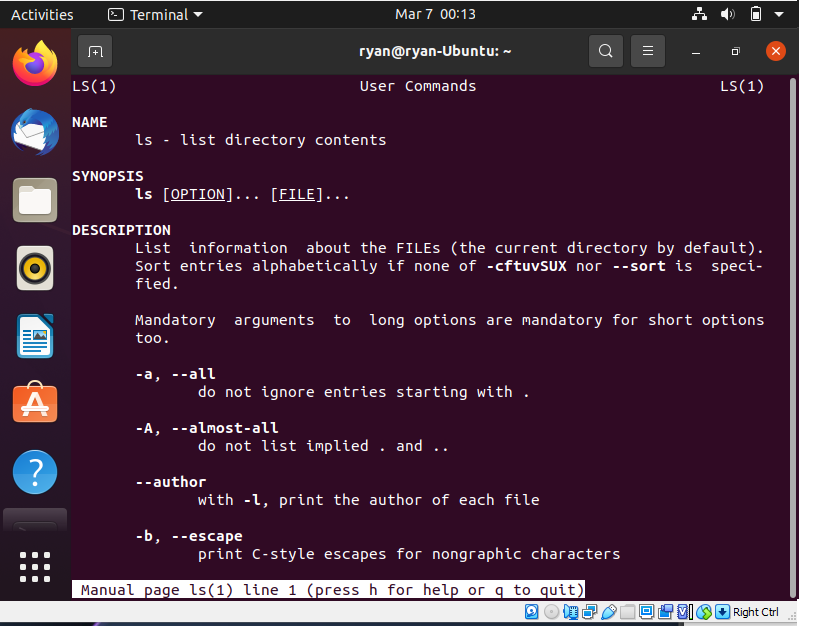
\includegraphics[width=0.5\textwidth]{Gambar/tut 1.2 man-ls.png}
    \caption{Man ls}
    \label{fig:my_label}
    \end{figure}

\subsection{Tut 1.3 Shell}
    Pada percobaan tut 1.3 menampilkan shell dengan menggunakan \textit{syntax} echo, dan menampilkan shell yang lagi aktif dengan output /bin/bash.
    \begin{figure}[h]
     \centering
    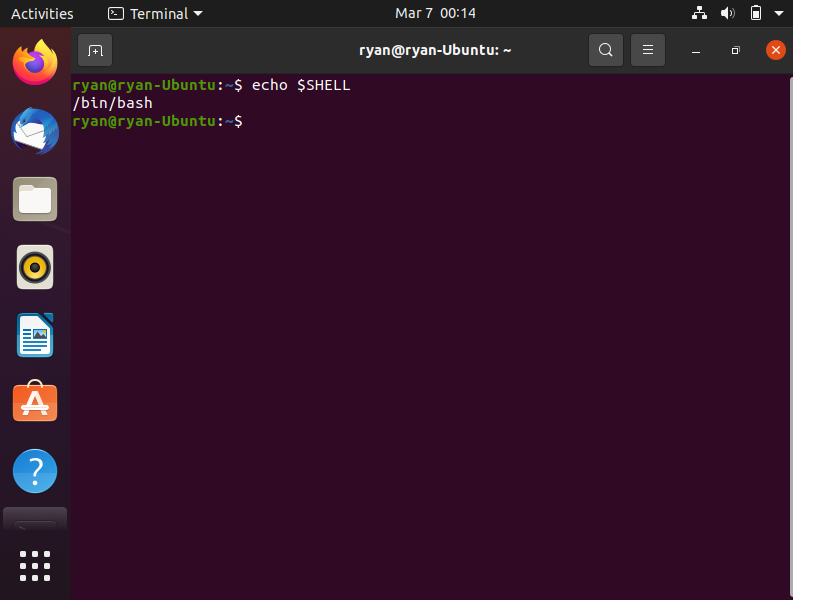
\includegraphics[width=0.5\textwidth]{Gambar/tut 1.3 echo-shell.png}
    \caption{Shell}
    \label{fig:my_label}
    \end{figure}
   \newpage
    
\subsection{Tut 1.4 Who, ls, cd, cat, mkdir, rmdir, rm, date, history, more, mv, cp, cal, pwd}
    Percobaan tut 1.4 ini melakukan beberapa percobaan perintah diantaranya yaitu who fungsinya untuk mengetahui atau melihatkan user yang sedang berjalan, mkdir fungsinya untuk membuat folder atau direktori baru, cp fungsinya untuk menyalin (copy) file, cd fungsinya untuk membuka atau mengubah direktori, ls fungsinya untuk menampilkan seluruh isi dalam direktori, rm fungsinya untuk menghapus (remove) file, rmdir fungsinya untuk menghapus (remove) direktori kosong, dan mv fungsinya untuk mengubah nama (rename) file, cal fungsinya untuk melihat calender, pwd fungsinya untuk print direktori yang aktif.

\begin{figure}[h]
	\centering
	\begin{subfigure}[b]{0.4\textwidth}
		\centering
		\def\svgwidth{\columnwidth}
		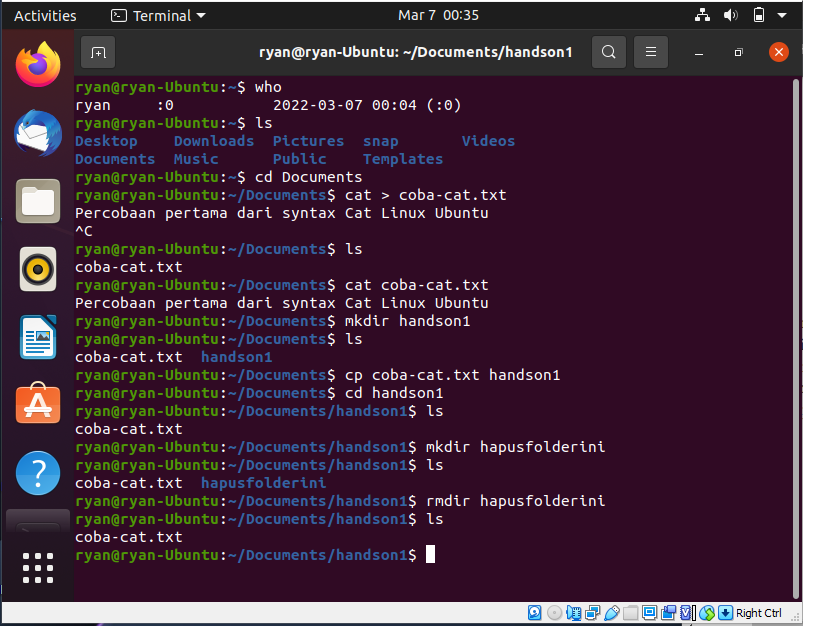
\includegraphics[width=0.8\textwidth]{Gambar/tut 1.4.1 echo-shell.png}
		\caption{who, ls, cd, cat, mkdir, cp, rmdir}
		\label{fig:aug-1}
	\end{subfigure}
	\qquad
	\begin{subfigure}[b]{0.4\textwidth}
		\centering
		\def\svgwidth{\columnwidth}
		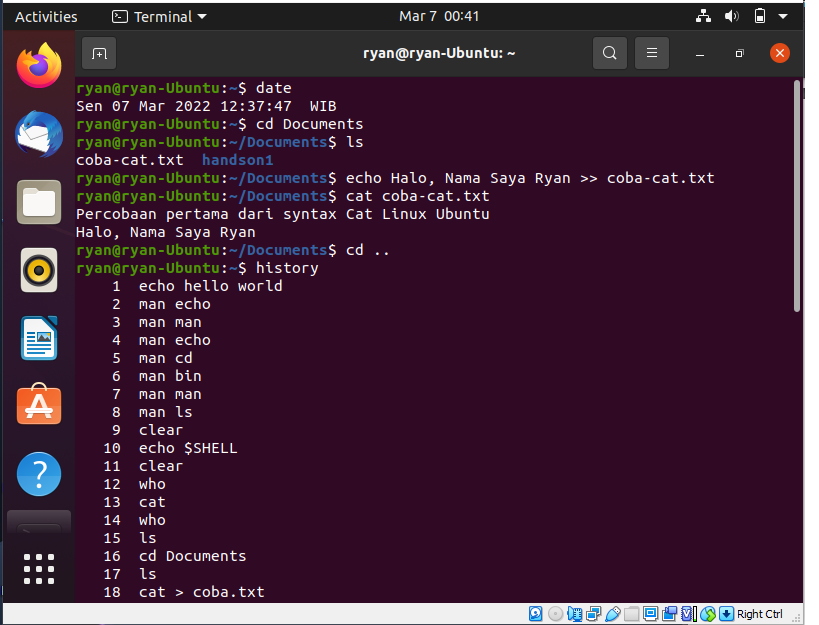
\includegraphics[width=0.8\textwidth]{Gambar/tut 1.4.2 echo-shell.png}
		\caption{date, echo, history}
		\label{fig:aug-2}
	\end{subfigure}
	\begin{subfigure}[b]{0.4\textwidth}
		\centering
		\def\svgwidth{\columnwidth}
		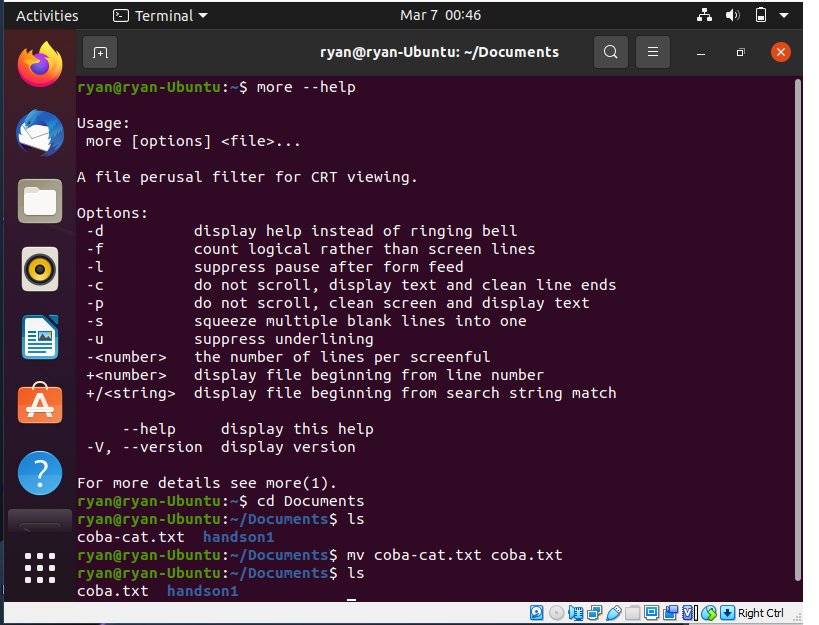
\includegraphics[width=0.8\textwidth]{Gambar/tut 1.4.3 echo-shell.png}
		\caption{more, mv}
		\label{fig:aug-2}
	\end{subfigure}
	\qquad
	\begin{subfigure}[b]{0.4\textwidth}
		\centering
		\def\svgwidth{\columnwidth}
		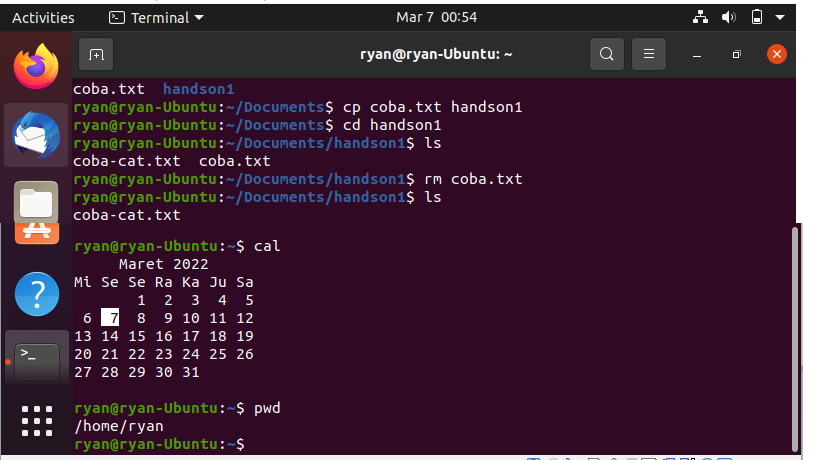
\includegraphics[width=1\textwidth]{Gambar/tut 1.4.4 echo-shell.png}
		\caption{cal, pwd}
		\label{fig:aug-2}
	\end{subfigure}
	\caption{Percobaan beberapa syntax}\label{fig:aug}
\end{figure}

\section{Laporan Percobaan Tut2}
\subsection{Tut 2.1 Sed}
    Percobaan tut 2.1 ini menjalankan \textit{syntax} sed. Pada sed pertama fungsinya untuk menghapus 1 karakter dari awal kalimat. Sed kedua fungsinya untuk menghapus 1 karakter di akhir kalimat. Sed ketiga saya mengalami error karena salah penulisan titik dua yang seharusnya ditulis dengan titik koma. Sed keempat fungsinya untuk menghapus 1 karakter diawal dan akhir kalimat. Karakter memang dihapus, tetapi tidak berpengaruh dalam isi pada file txt.
    \begin{figure}[h]
    \centering
    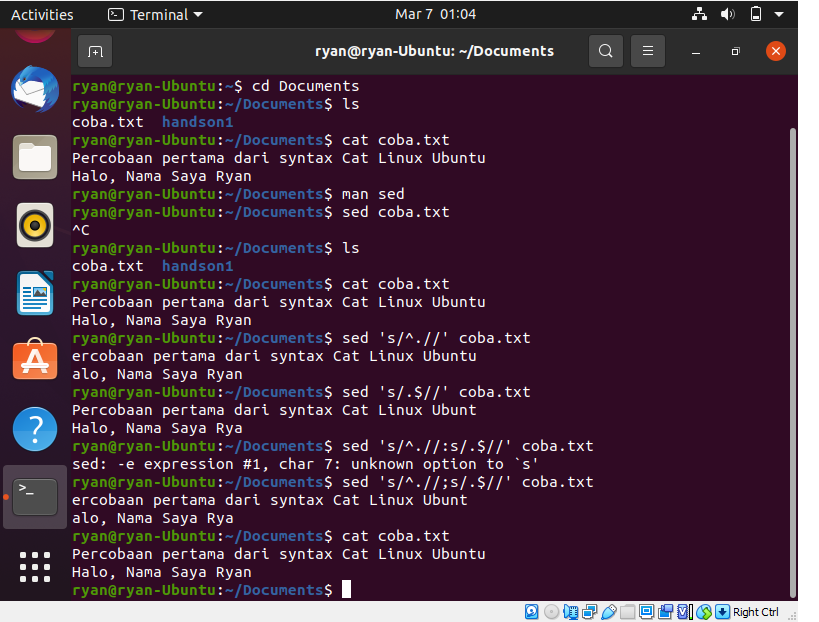
\includegraphics[width=0.5\textwidth]{Gambar/tut 2.1 sed.png}
    \caption{Sed}
    \label{fig:my_label}
    \end{figure}

\subsection{Tut 2.2 Grep}
    Pada tut 2.2 ini menjalankan \textit{syntax} grep yang berfungsi mencari kata di sebuah kalimat yang biasanya ditandai dengan warna merah pada kalimat yang dicari. Pada \textit{syntax} grep -c ini berfungsi untuk menghitung banyaknya kata pada baris kalimat dan menampilkan jumlah dari kata tersebut.
    \begin{figure}[h]
    \centering
    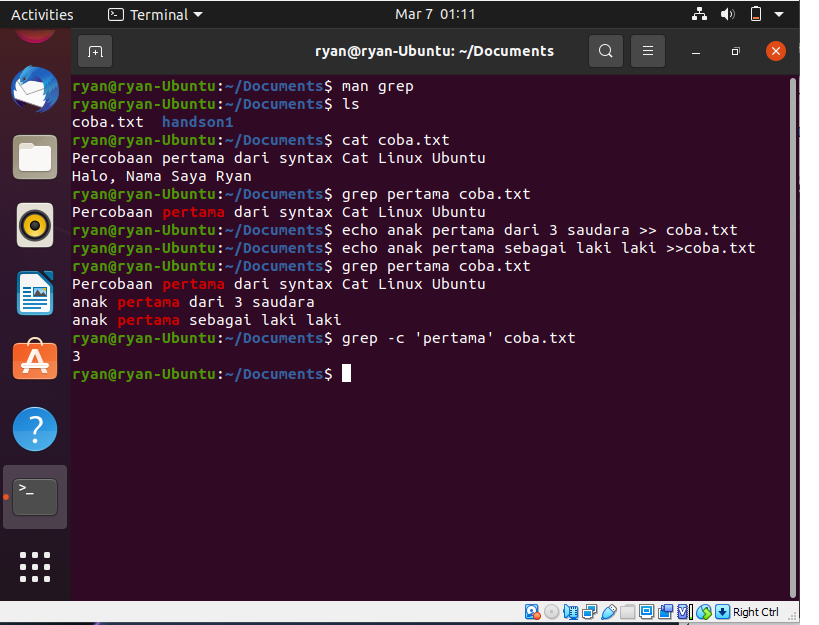
\includegraphics[width=0.5\textwidth]{Gambar/tut 2.2 grep.png}
    \caption{Grep}
    \label{fig:my_label}
    \end{figure}
    
\section{Laporan Percobaan Tut3}
\subsection{Tut 3.1 Shell Script Display}
    Pada tut3 ini menjalankan \textit{syntax} nano yang berfungsi untuk membuat dan membuka open editor shell skrip dengan format file sh. Dalam \textit{script} shell, saya menuliskan \textit{syntax} echo "HELLO WORLD" yang kemudian saya simpan. Untuk \textit{syntax} Sh disini fungsinya untuk memanggil file yang dibuat dan akan menampilkan isi dari file, sama seperti \textit{syntax} './'. Pada \textit{syntax} chmod 777 disini file test.sh berubah izinnya menjadi publik dan biasanya berwarna hijau, sedangkan chmod 600 merubah file test.sh menjadi private.
    \begin{figure}[h]
	\centering
	\begin{subfigure}[b]{0.4\textwidth}
		\centering
		\def\svgwidth{\columnwidth}
		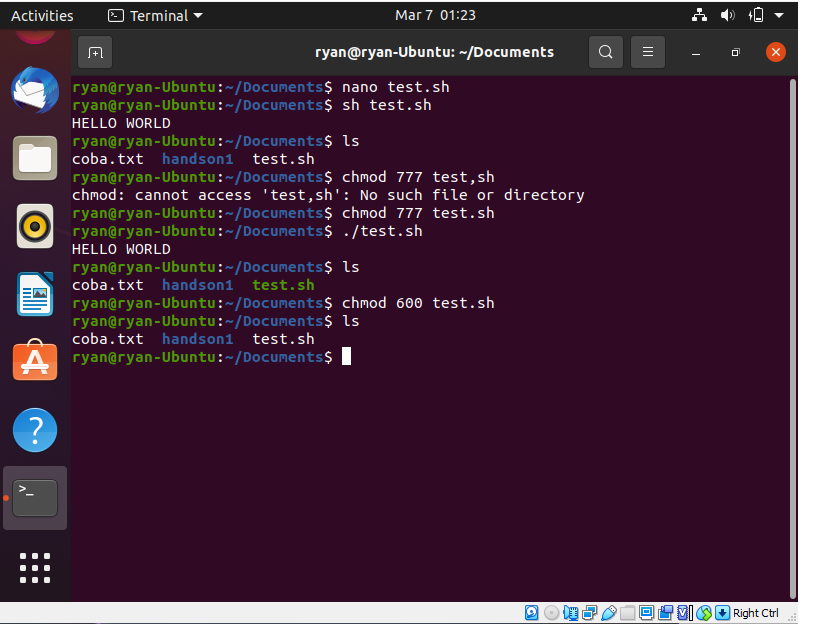
\includegraphics[width=1\textwidth]{Gambar/tut 3 shell command.png}
		\caption{Shell nano, chmod}
		\label{fig:aug-1}
	\end{subfigure}
	\qquad %add desired spacing between images, e. g. ~, \quad, \qquad, \hfill etc. 
	%(or a blank line to force the subfigure onto a new line)
	\begin{subfigure}[b]{0.4\textwidth}
		\centering
		\def\svgwidth{\columnwidth}
		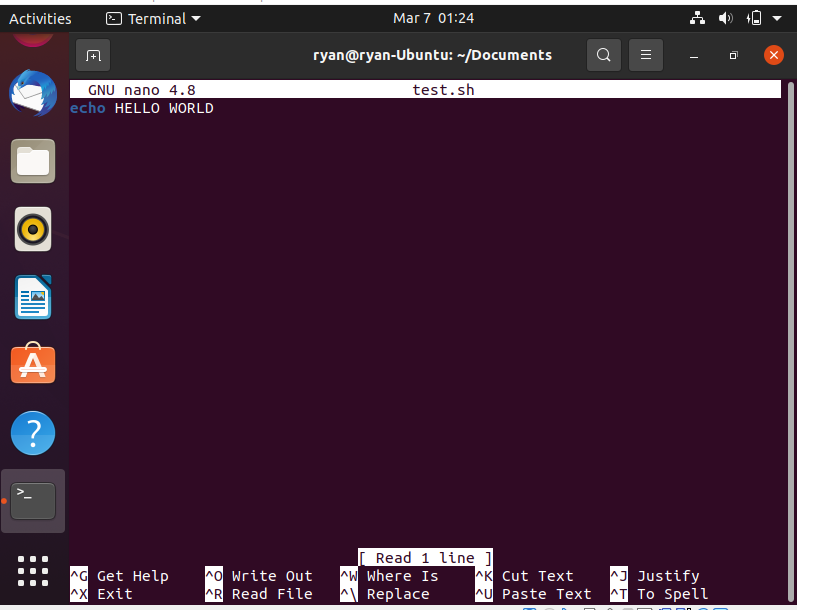
\includegraphics[width=1\textwidth]{Gambar/tut 3 shell script.png}
		\caption{Shell Script Command}
		\label{fig:aug-2}
	\end{subfigure}
	\caption{Shell Script Display}\label{fig:aug}
\end{figure}

\section{Laporan Pembahasan Tugas(6)}
    Pada \textit{assignment 6 user} diminta untuk mengubah kalimat dari huruf kecil menjadi kalimat huruf besar. Disini saya membuat file dengan terminal dan \textit{syntax} nano dengan format sh, kemudian teks tersebut akan dipanggil. Percobaan ini memerlukan 2 file yaitu dengan format .sh dan .txt. File dengan format .sh berisi code dengan menggunakan \textit{syntax} echo dan berfungsi sebagai output teks, \textit{syntax} read berfungsi untuk membaca file yang saya buat yaitu dengan format .txt. file 2 berisi kalimat yang nantinya akan diubah dari karakter kecil menjadi karakter besar.
    
    \begin{figure}[h]
	\centering
	\begin{subfigure}[b]{0.4\textwidth}
		\centering
		\def\svgwidth{\columnwidth}
		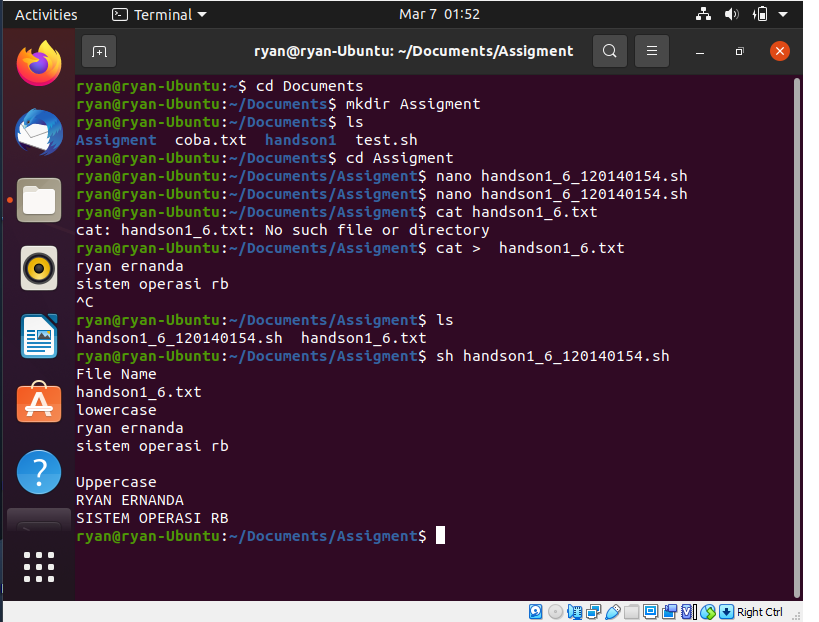
\includegraphics[width=1\textwidth]{Gambar/Assigment 6 command.png}
		\caption{Shell nano}
		\label{fig:aug-1}
	\end{subfigure}
	\qquad %add desired spacing between images, e. g. ~, \quad, \qquad, \hfill etc. 
	%(or a blank line to force the subfigure onto a new line)
	\begin{subfigure}[b]{0.4\textwidth}
		\centering
		\def\svgwidth{\columnwidth}
		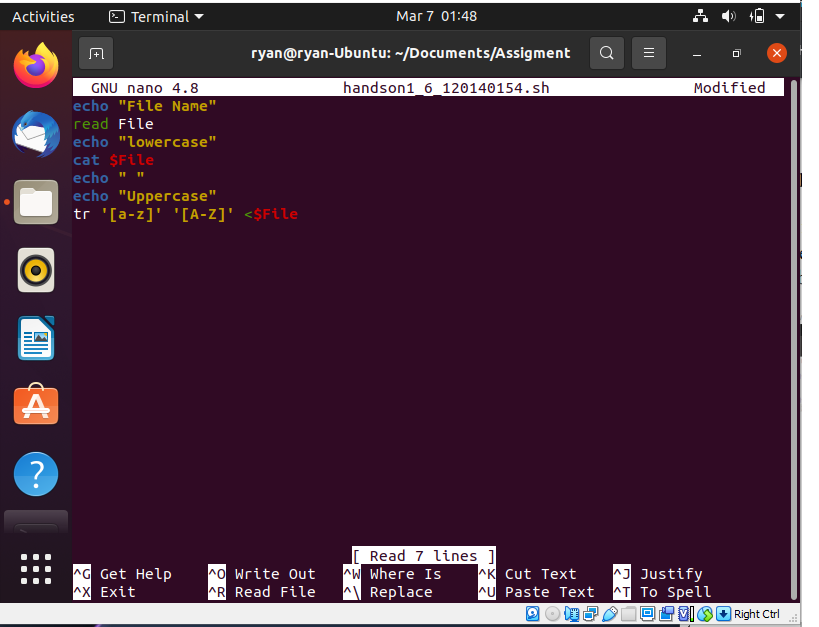
\includegraphics[width=1\textwidth]{Gambar/Assigment 6 shell.png}
		\caption{Shell Script Command}
		\label{fig:aug-2}
	\end{subfigure}
	\caption{Mengubah \textit{Lowercase} menjadi \textit{Uppercase}}\label{fig:aug}
\end{figure}
    
\section{Laporan Pembahasan Tugas(8)}
    Pada \textit{assigment 8 user} diminta menuliskan shell skrip yang menerima file, baris awal dan akhir sebagai kalimat dan menampilkan semua baris yang diberikan angka. Dalam percobaan ini memerlukan 2 file dengan format .sh dan .txt. File 1 berisikan code dengan menggunakan terminal dan \textit{syntax} echo berfungsi sebagai output teks, \textit{syntax read} digunakan sebagai input kata yang ditulis, \textit{syntax sed} berfungsi untuk menghapus baris yang tidak ingin ditampilkan, \textit{syntax cat} berfungsi untuk membuka isi file. file 2 berisi beberapa kalimat yang ditampilkan ketika baris awal dan baris akhir ditentukan.
    \begin{figure}[h]
	\centering
	\begin{subfigure}[b]{0.4\textwidth}
		\centering
		\def\svgwidth{\columnwidth}
		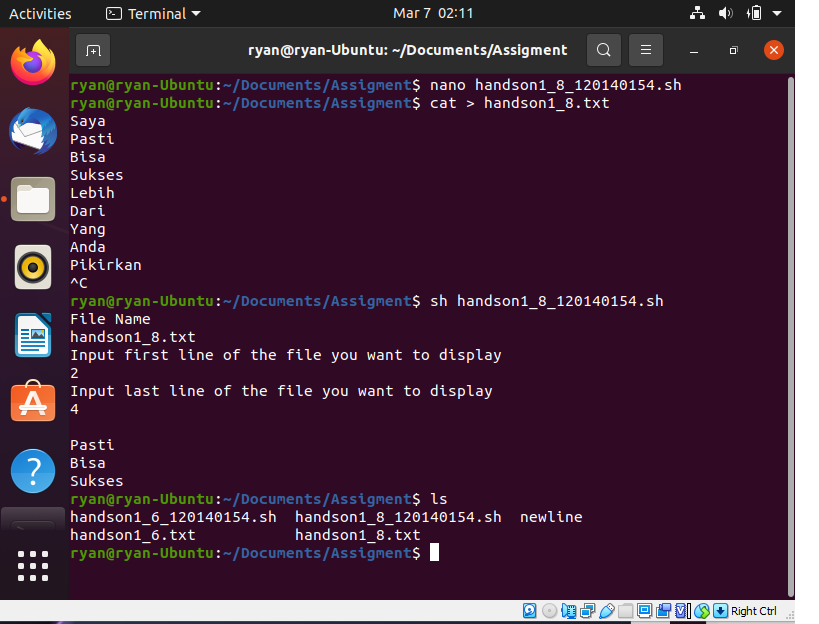
\includegraphics[width=1\textwidth]{Gambar/Assigment 8 command.png}
		\caption{Shell nano}
		\label{fig:aug-1}
	\end{subfigure}
	\qquad %add desired spacing between images, e. g. ~, \quad, \qquad, \hfill etc. 
	%(or a blank line to force the subfigure onto a new line)
	\begin{subfigure}[b]{0.4\textwidth}
		\centering
		\def\svgwidth{\columnwidth}
		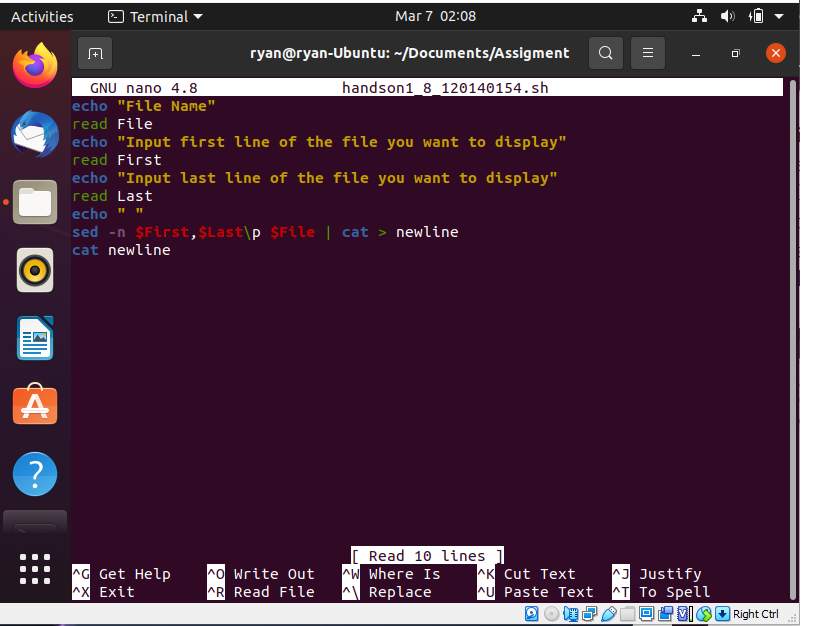
\includegraphics[width=1\textwidth]{Gambar/Assigment 8 shell.png}
		\caption{Shell Script Command}
		\label{fig:aug-2}
	\end{subfigure}
	\caption{Menghapus Kalimat Sesuai Baris}\label{fig:aug}
\end{figure}

\section{Laporan Pembahasan Tugas(9)}
    Pada \textit{assigment 8, user} diminta untuk menulis shell skrip digunakan untuk menghapus semua baris dan memiliki kata yang sama dalam file yang disediakan sabagai argumen. Dalam percobaan ini memerlukan 2 file dengan format .sh dan .txt. File 1 berisikan code menggunakan perintah echo berfungsi sebagai keluaran teks, \textit{syntax read} digunakan sebagai input kata yang ditulis, terminal grep yang berfungi menghapus kalimat jika dalam kalimat tersebut terdapat kalimat yang sama. file 2 berisi kalimat dalam beberapa baris dan terdapat kalimat yang sama.
    \begin{figure}[h]
	\centering
	\begin{subfigure}[b]{0.4\textwidth}
		\centering
		\def\svgwidth{\columnwidth}
		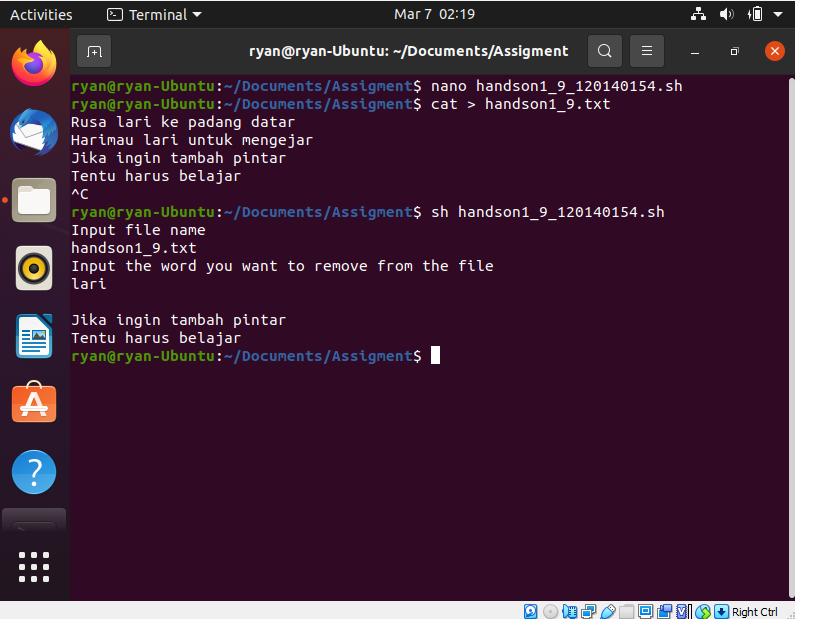
\includegraphics[width=1\textwidth]{Gambar/Assigment 9 command.png}
		\caption{Shell nano}
		\label{fig:aug-1}
	\end{subfigure}
	\qquad %add desired spacing between images, e. g. ~, \quad, \qquad, \hfill etc. 
	%(or a blank line to force the subfigure onto a new line)
	\begin{subfigure}[b]{0.4\textwidth}
		\centering
		\def\svgwidth{\columnwidth}
		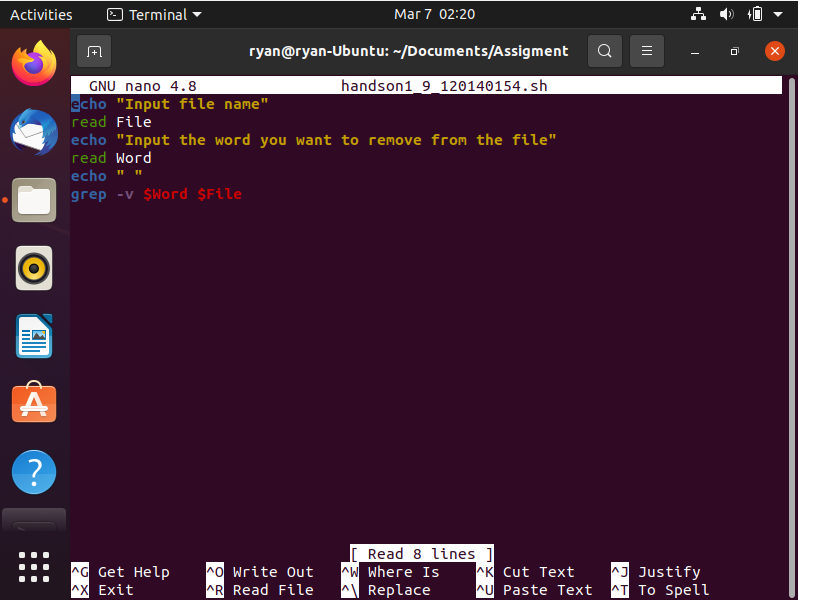
\includegraphics[width=1\textwidth]{Gambar/Assigment 9 shell.png}
		\caption{Shell Script Command}
		\label{fig:aug-2}
	\end{subfigure}
	\caption{Menghapus Kalimat yang Sama}\label{fig:aug}
\end{figure}

\section{Kesimpulan}
     Yang dapat saya simpulkan dalam menyelesaikan tugas HandsOn 1 ini yaitu saya belajar dan memahami beberapa perintah dalam linux serta fungsinya. Tidak hanya itu saya juga bisa mengerjakan laporan dengan menggunakan latex online overleaf, ini merupakan hal yang baru bagi saya karna saya bisa mengerjakan laporan sambil memodifikasi perintah perintah dalam latex ini.
     
\section{Link Google Drive}
Link Folder Assigment HandsOn 1 : \href{https://drive.google.com/drive/folders/1lQRKM7aLH1yirpGWvwh2ChhqQv5B_60c?usp=sharing}{Klik Disini}.

\end{document}